\documentclass{beamer}
\usetheme{Antibes}
\usepackage{amsmath, amsfonts, amssymb}
\usepackage{physics}
\setbeamertemplate{footline}[frame number]

\DeclareMathOperator*{\argmin}{arg\,min}

\title{Solving the Wide-band Inverse Scattering Problem via Equivariant Neural Networks}
\subtitle{Borong Zhang, Leonardo Zepeda-Nunez, Qin Li}
\author{Presented by: Alexander Hsu, Evgenii Samutichev}

\begin{document}

\maketitle

\begin{frame}{Outline}
    \tableofcontents
\end{frame}

\section{Problem setup}

\subsection{Forward problem}
\begin{frame}{Forward problem}
    \begin{itemize}
        \item Helmholtz equation setting, domain of interest $\Omega$, Sommerfeld radiation condition
        \item The media is described by $\eta(\mathbf{x}) = n(\mathbf{x}) - 1$ where $n$ is the refractive index
        \item Probing wave $u^{\text{in}} = e^{i \omega \mathbf{s} \cdot \mathbf{x}}$ of frequency $\omega$ and direction $\mathbf{s} \in \mathbb{S}^1$ triggers the scattered wave field $u^{\text{sc}}(\mathbf{x}; \mathbf{s})$
    \end{itemize}
    
    \begin{equation}
        \Delta u^{\text{sc}} (\mathbf{x}) + \omega^2 (1 + \eta(\mathbf{x})) u^{\text{sc}}(\mathbf{x}) = -\omega^2 \eta(\mathbf{x}) u^{\text{in}}(\mathbf{x})
    \end{equation}

    \begin{columns}[T] % align columns
        \begin{column}{.48\textwidth}
            \begin{figure}
                \centering
                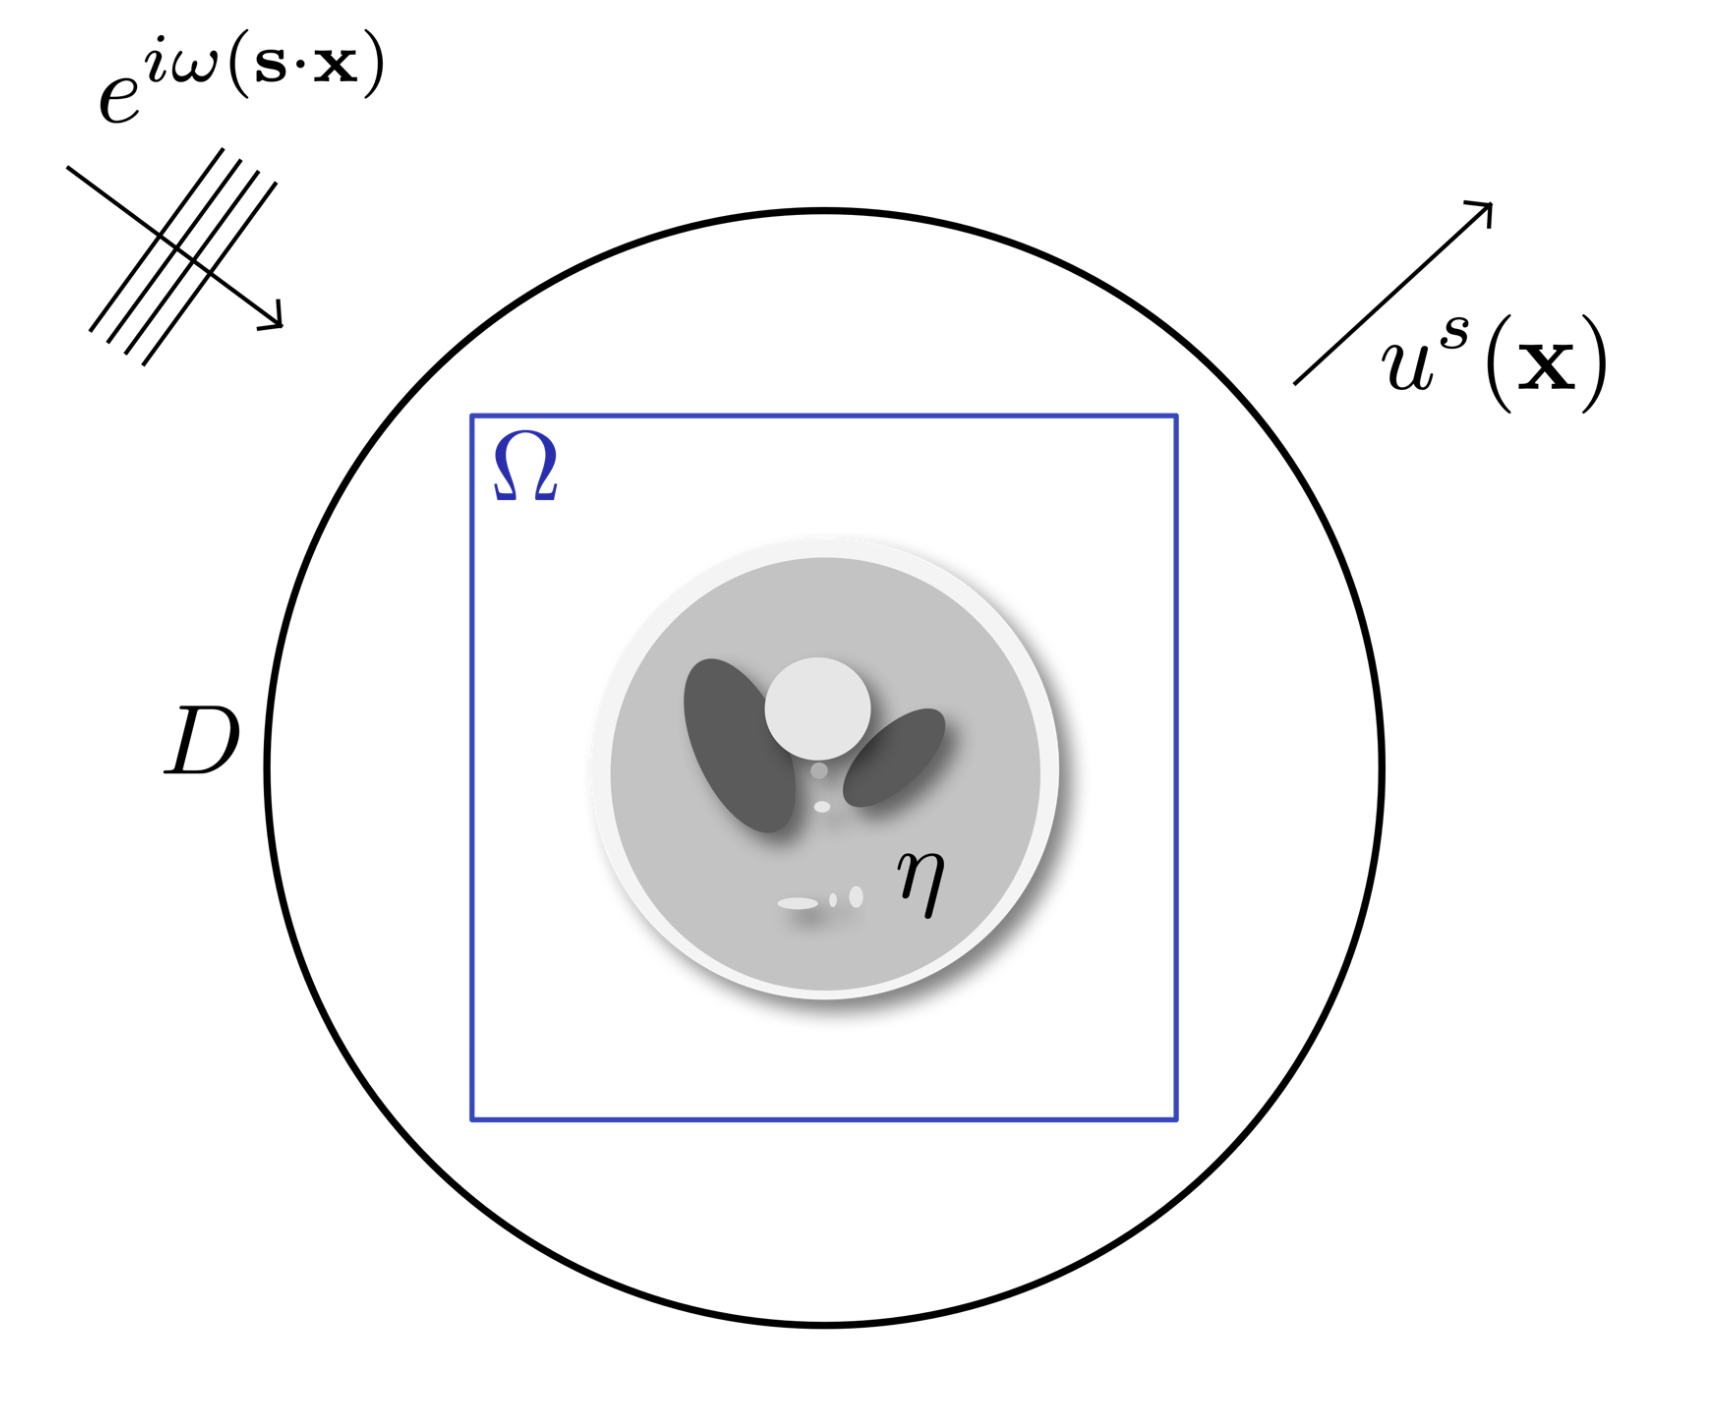
\includegraphics[width=0.70\textwidth]{images/Wave propagation.png}
                \label{fig:enter-label}
            \end{figure}
        \end{column}%
        \hfill%
        \begin{column}{.48\textwidth}
            The measurements are taken on the circle $D$ of radius $R$:
            $$\Lambda^\omega (\mathbf{s}, \mathbf{r}) = u^{\text{sc}}(R \mathbf{r}; \mathbf{s})$$
            $$\textbf{FP:} \ \Lambda^\omega = \mathcal{F}^\omega [\eta]$$
        \end{column}%
        \end{columns}
\end{frame}

\subsection{Inverse problem}
\begin{frame}{Inverse problem}

\begin{itemize}
    \item The \textbf{inverse problem} is to infer the media $\eta$ from the measured data $\{\Lambda^{\omega}\}_{\omega \in \bar{\Omega}}$ where $\bar{\Omega}$ is a set of frequencies
    \begin{equation}
        \eta^* = \mathcal{F}^{-1}(\{\Lambda^{\omega}\}_{\omega \in \bar{\Omega}})
    \end{equation}
    \item A classical way is to recast this problem to PDE-constrained optimization
    \begin{equation}
        \eta^* = \argmin_{\nu}{\sum_{\omega \in \bar{\Omega}}{\norm{\mathcal{F}^\omega[\nu] - \Lambda^\omega }^2}}
    \end{equation}
    which can be solved by highly tailored gradient-descent optimization techniques.
\end{itemize}

\section{Theory behind the model}
\subsection{Properties of forward/inverse map}
\end{frame}

\subsection{Linearization}
\begin{frame}{Linearization}
    \begin{itemize}
        \item Perturbation of the input $\eta = \eta_0 + \delta \eta$ 
        \begin{align*}
            \mathcal{F}^\omega [\eta] &= \mathcal{F}^\omega [\eta_0 + \delta \eta] \approx \mathcal{F}^\omega [\eta_0] + F^\omega \delta \eta  \\
            \Lambda^\omega &= \mathcal{F}^\omega [\eta ] \approx F^\omega \eta
        \end{align*}
        \item Born approximation
        \begin{equation}
            (F^\omega\eta)(\mathbf{s}, \mathbf{r}) = C_{norm} \int_{\Omega}{e^{-i\omega (\mathbf{r} - \mathbf{s})\cdot \mathbf{y}} \eta(\mathbf{y}) d\mathbf{y}}
        \end{equation}
        \item Involves very oscillatory integrals
        \item In this setting, the data $\Lambda^\omega$ can be viewed as a first-type Fredholm integration over $\eta$
    \end{itemize}
\end{frame}

\subsection{Filtered back-projection}
\begin{frame}{Filtered back-projection}
\begin{itemize}
    \item Now, for the inverse problem we search for a solution $\eta^*$ to the following optimization problem
    \begin{equation}
        \min _\eta\left\|\Lambda^\omega-F^\omega \eta\right\|^2  + \epsilon \norm{\eta}^2
    \end{equation}
    where 
    \begin{equation}
        \left\|\Lambda^\omega-F^\omega \eta\right\|^2=\int_{\mathbb{S}^1 \times \mathbb{S}^1}\left|\Lambda^\omega(\boldsymbol{s}, \boldsymbol{r})-\left(F^\omega \eta\right)(\boldsymbol{s}, \boldsymbol{r})\right|^2 d \boldsymbol{r} d \boldsymbol{s}
    \end{equation}
    \item The solution is explicitly given by 
    \begin{equation}
        \eta^* = ((F^\omega)^* F^\omega + \epsilon I)^{-1} (F^\omega)^* \Lambda^\omega
    \end{equation}
    \item This formula isn't valid when real $\eta$ is significant, and only serves as a guidance for the actual inversion.
    
\end{itemize}
    
\end{frame}

\subsection{Structure of input and output data}
\begin{frame}{Structure of input and output data}
    \begin{itemize}
        \item $n_{freq}$ frequencies. Again, in theory, one should be enough if we had complete perfect info.
        \item Each has $n_{obs}$ source directions and observation points
        \item Probe with $n_{obs}$ directions $s$, and then observe $u^{\text{sc}}(R \mathbf{r}; \mathbf{s})$ at $n$ points $r$ on the circle.
        
    \end{itemize}
\end{frame}

\subsection{Equivariance}
\begin{frame}{Equivariance (1 / 2)}
    \begin{itemize}
        \item Remember filtered back-projection
        \begin{equation}
            \eta^* = ((F^{\omega})^* F^\omega + \epsilon I)^{-1} (F^\omega)^* \Lambda^\omega
        \end{equation}
        \item Back-scattering operator  $(F^\omega)^*$ is rotation equivariant, and naturally represented on the polar coordinates
        \item Filtering operator $((F^\omega)^* F^\omega + \epsilon I)^{-1}$ is translation equivariant, and naturally represented on a Cartesian grid
        \item There is a function $p(\mathbf{x})$ s.t.
        \begin{equation}
            (F^\omega)^* F^\omega (\eta) = p * \eta
        \end{equation}
        \item The proposed strategy is to encode this into a convolutional neural network, including coordinate transformations
    \end{itemize}
\end{frame}

\begin{frame}{Equivariance (2 / 2)}
Rotational equivariance
    \begin{equation*}
    \left((F^\omega)^\ast \Lambda^\omega(r-a,s-a)\right) (\theta, \rho) =  [(F^\omega)^\ast \Lambda^\omega](\theta - a, \rho)\
\end{equation*}
Translational equivariance
\begin{equation}
\begin{aligned}
    (F^\omega)^\ast F^\omega[\eta](\bm{y}) &= \int_{[0,2\pi]^2} e^{i\omega(\bm{r}-\bm{s})\cdot \bm{y}} \left (\int_{\Omega} e^{-i\omega(\bm{r}-\bm{s})\cdot \bm{x}}\, \eta(\bm{x})\,d\bm{x} \right ) \, \,ds\,dr\,,\\
    &= \int_{[0,2\pi]^2}\int_{\mathbb{R}^2} e^{i\omega(\bm{r}-\bm{s})\cdot \bm{y}} e^{-i\omega(\bm{r}-\bm{s})\cdot \bm{x}}\, \eta(\bm{x})\,d\bm{x}\, \,ds\,dr\,,\\
    &= \int_{\mathbb{R}^2} \left (\int_{[0,2\pi]^2}e^{i\omega(\bm{r}-\bm{s})\cdot (\bm{y}-\bm{x})} \,ds\,dr\,\right ) \, \eta(\bm{x})\,d\bm{x}\,,\\
    & = \int p(\bm{y}-\bm{x})\eta(\bm{x})d\bm{x} = p\ast \eta(\bm{y}).\\
\end{aligned}
\end{equation}


\end{frame}

\subsection{Application of rotation equivariance}
\begin{frame}{Application of rotation equivariance computing backscattering...}
\[
\mathsf{K}^\omega \in \R^{n_\sca\times n_\rho}\,,\quad\text{with}\quad \mathsf{K}^\omega_{mn} = e^{-i\omega\rho_n\cos(t_m)} = K^\omega(\rho_n,t_m)\,.
\]
\begin{align*}
\alpha^\omega(\theta_j,\cdot) &= \sf((F^\omega)^*\Lambda^\omega)(\theta_j,\cdot) \\
&= \operatorname{ones}(1,n_{source})\cdot [\barr{\mathsf{K}^\omega} \odot (\sf\Lambda^\omega_{\theta_j}\cdot \mathsf{K}^\omega )] \\
&= \operatorname{diag}[(\mathsf{K}^\omega)^\ast \cdot \sf\Lambda^\omega_{\theta_j}\cdot \mathsf{K}^\omega]
\end{align*}
\end{frame}

\section{CNN architecture and results}
\subsection{Wide-Band Equivariant Network}
\begin{frame}{Wide-Band Equivariant Network}
    \begin{enumerate}
        \item Compute the discretized back-scattering $\alpha^\omega(\theta, \rho) := (F^\omega)^*\Lambda^\omega$ for each frequency $\omega \in \bar{\Omega}$, 
        \item Coordinate transformation $\alpha^\omega (\theta, \rho)$ to $\alpha^\omega (x,y)$ using polynomial interpolation
        \item Feedforward to the CNN that approximates the filtering operator $((F^\omega)^* F^\omega + \epsilon I)^{-1}$
    \end{enumerate}
    \begin{figure}
        \centering
        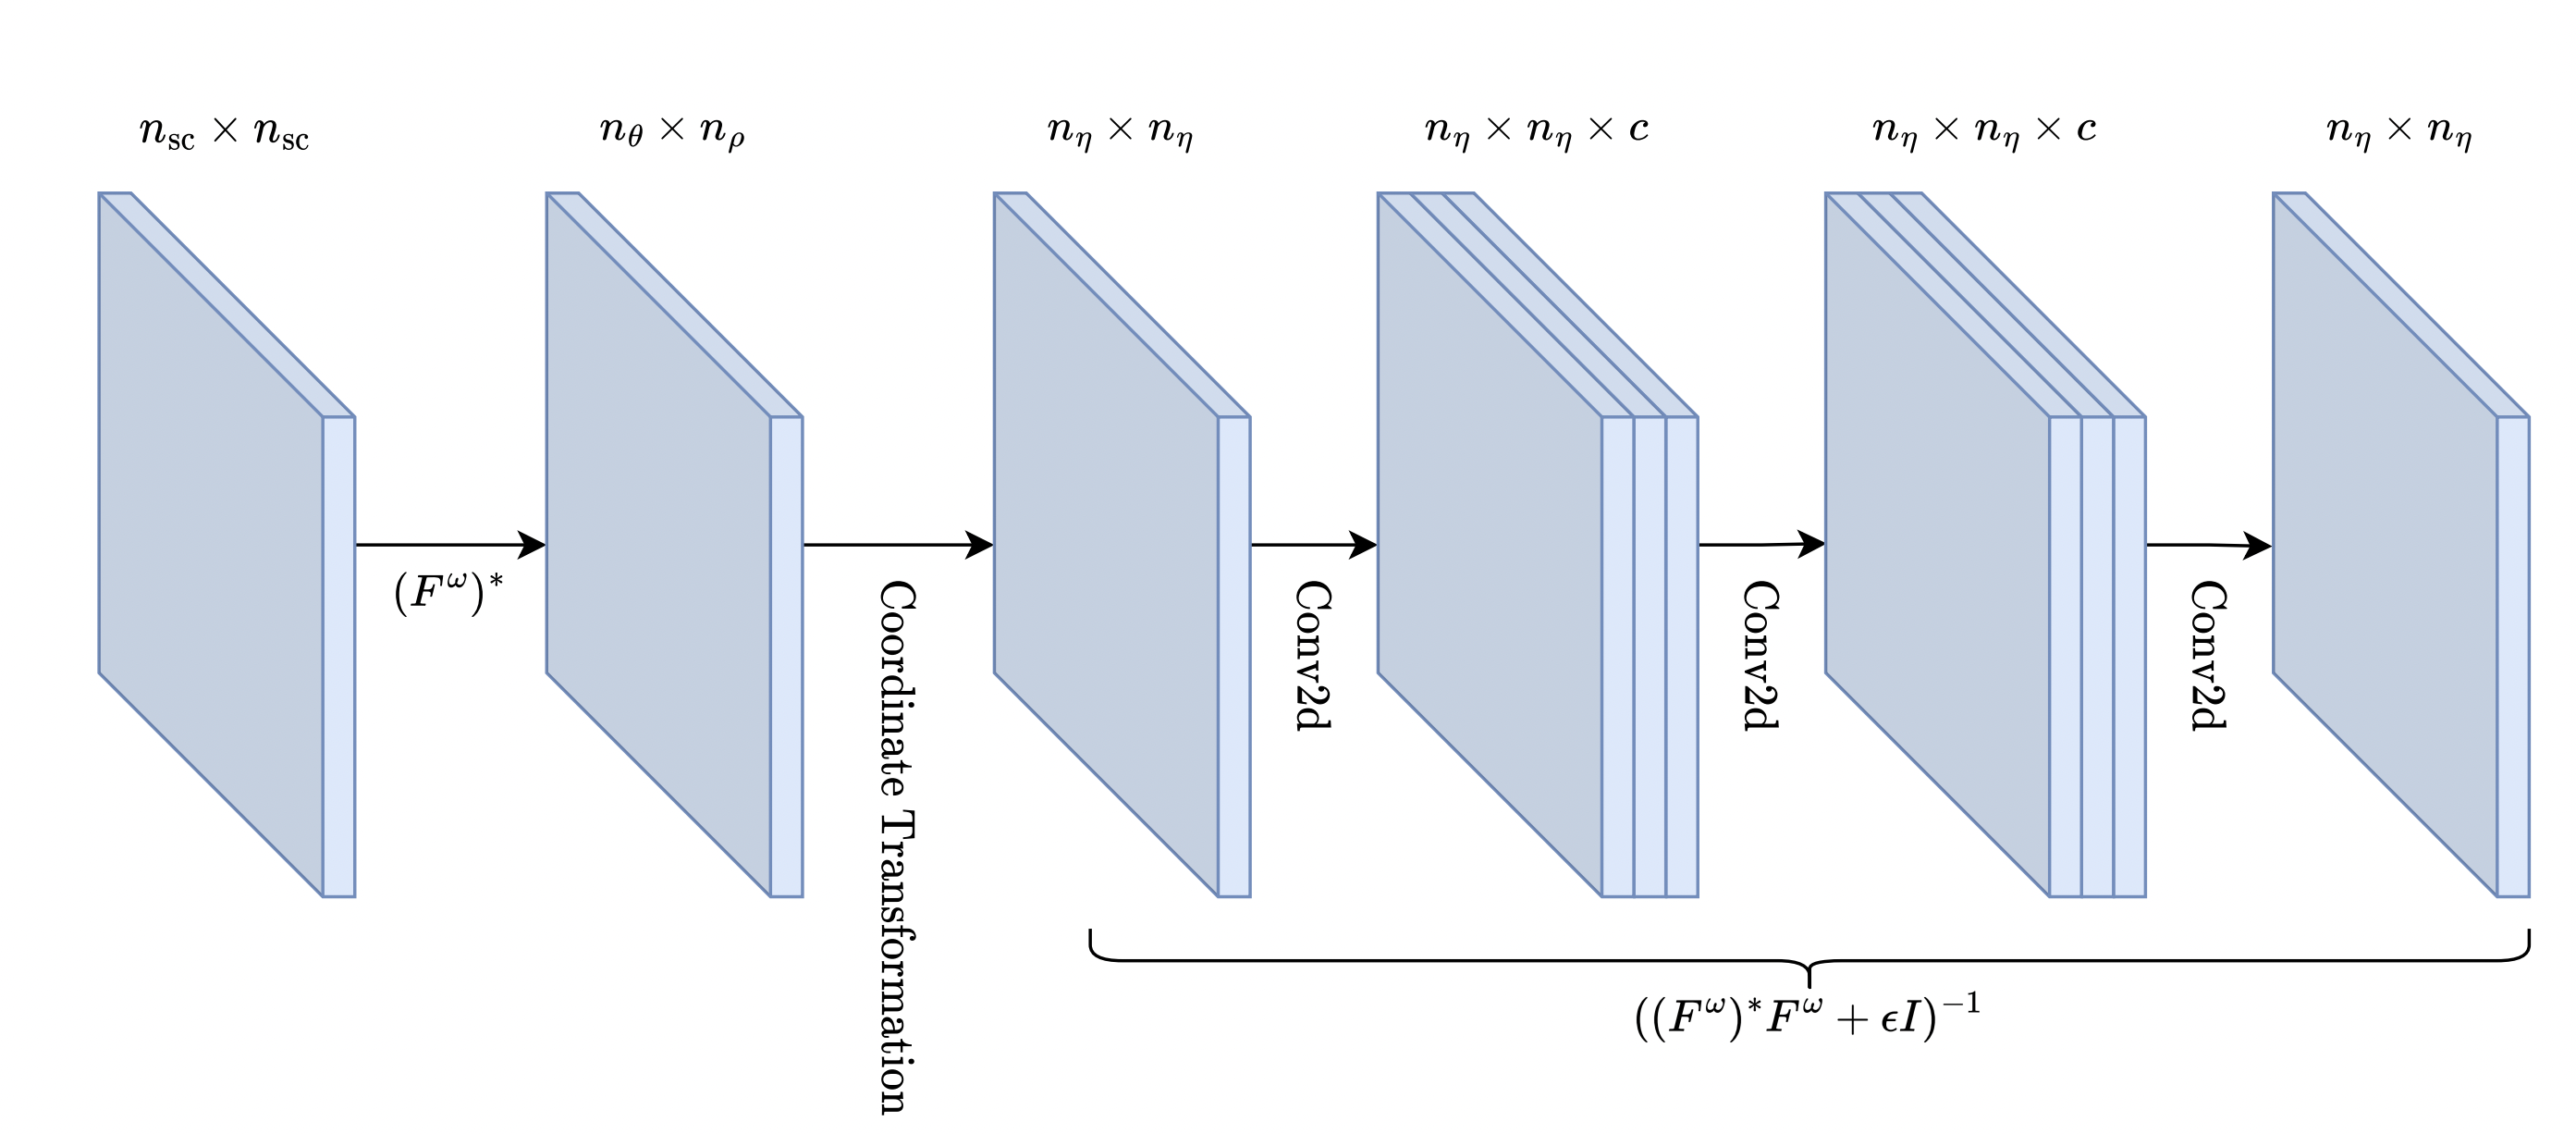
\includegraphics[width=0.7\textwidth]{images/CNN.png}
    \end{figure}
\end{frame}

\subsection{Training dataset}
\begin{frame}{Training dataset}
    \begin{itemize}
        \item Media + corresponding wide-band far-field patterns at three different frequencies $2.5, 5$ and $10$ Hz, computed using finite-differences
        \item Picked $n_\eta = 80$, so the resolution of the media is $80 \times 80$
        \item $n_\text{sc} = 80$ equiangular recievers and sources
        \item Model was trained for each of 5 categories of media
        \begin{itemize}
            \item Shepp-Logan phantom, representing a human head
            \item  Random smooth perturbations
            \item Triangles of sizes 10, 5, 3, randomly located and oriented
        \end{itemize}
    \end{itemize}
    \begin{figure}
        \centering
        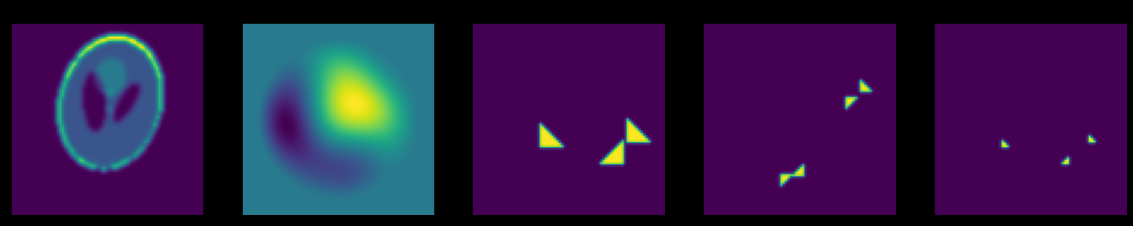
\includegraphics[width=0.8\textwidth]{images/data.png}
    \end{figure}
\end{frame}

\subsection{Training procedure}
\begin{frame}{Training procedure}
    \begin{itemize}
        \item Let's denote our network as 
        \begin{equation}
            \eta = \Phi_\Theta (\{\Lambda^\omega\}_{\omega \in \bar{\Omega}})
        \end{equation}
        \item Then, we train it by minimizing the MSE
        \begin{equation}
            \min_{\Theta}{\frac{1}{N_s}\sum_{s=1}^{N_s}\left\|\Phi_{\Theta}(\{\Lambda^{\omega,[s]}\}_{\omega \in \bar{\Omega}})-\eta^{[s]}\right\|^2}
        \end{equation}
        \item Adam optimizer with learning rate $3 \times 10^{-4}$
        \item Batch size $16$
        \item Exponential scheduler 
        \item 100 epochs
    \end{itemize}
\end{frame}

\subsection{Performance}
\begin{frame}{Performance (1 / 2)}
    \begin{itemize}
        \item The model was compared by relative RMSE with Wide-band Butterfly Network (WBBN) and Fourier Neural Operator (FNO) models
    \end{itemize}
    \begin{figure}
        \centering
        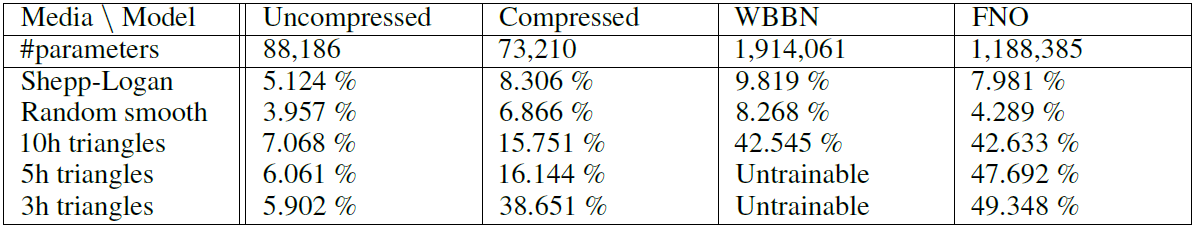
\includegraphics[width=\textwidth]{images/Comparison.png}
    \end{figure}
\end{frame}

\begin{frame}{Performance (2 / 2)}
    \begin{figure}
        \centering
        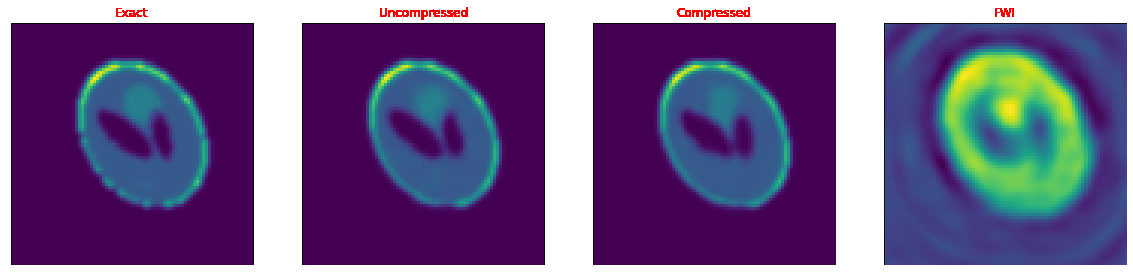
\includegraphics[width=0.7\textwidth]{images/comp1.png}
    \end{figure}
    \begin{figure}
        \centering
        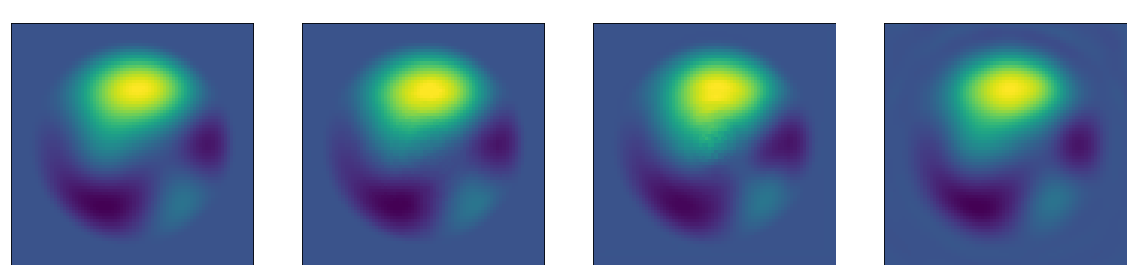
\includegraphics[width=0.7\textwidth]{images/comp3.png}
    \end{figure}
    \begin{figure}
        \centering
        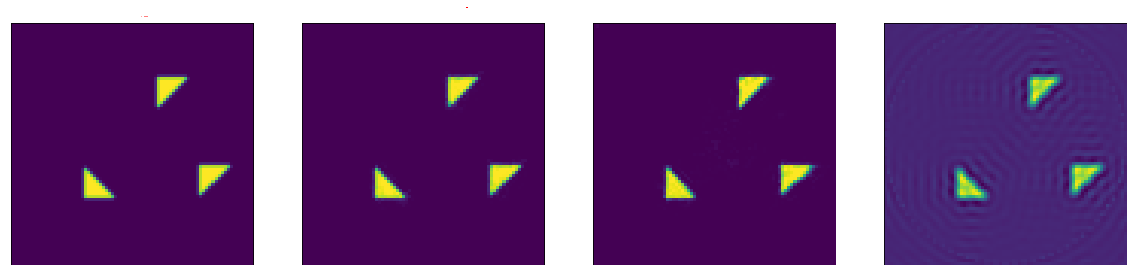
\includegraphics[width=0.7\textwidth]{images/comp2.png}
    \end{figure}
\end{frame}



\end{document}